\documentclass[10pt]{article}
\usepackage[margin=0.7in]{geometry}
\usepackage[T1]{fontenc}
\usepackage{mathptmx}
\usepackage{graphicx}
\usepackage{booktabs}
\usepackage{xcolor}
\usepackage[hidelinks]{hyperref}
\setlength{\parskip}{3pt}
\setlength{\parindent}{0pt}
\setlength{\textfloatsep}{8pt plus 2pt minus 2pt}
\setlength{\floatsep}{6pt plus 2pt minus 2pt}
\setlength{\intextsep}{6pt plus 2pt minus 2pt}
\setlength{\abovecaptionskip}{4pt}
\setcounter{topnumber}{3}
\setcounter{bottomnumber}{2}
\setcounter{totalnumber}{5}
\renewcommand{\topfraction}{0.85}
\renewcommand{\bottomfraction}{0.5}
\renewcommand{\textfraction}{0.1}
\renewcommand{\floatpagefraction}{0.8}

\title{\vspace{-2.2em}\large\textbf{Fundamental Stock Selection on the Point-in-Time S\&P 500:\\ Bias Audit and Backtest}\vspace{-0.6em}}
\author{\normalsize Alisa He (jh5111) \quad GR5398 Assignment 1, FinRL-Trading track}
\date{\normalsize October 12, 2026\vspace{-1.2em}}

\begin{document}
\maketitle

\begin{abstract}
\noindent The course FinRL-Trading pipeline was run end to end, and the equal-weight baseline was
reproduced: a final NAV of 1.31, against 2.55 for SPY. Further investigation shows that most of the
gap to SPY came from the backtest, not from the stock selection itself. The main issue is that the
backtest does not account for overnight returns. Three other problems also needed fixing: a
survivorship leak in the price table, a warm-up period with almost no live signals, and two look-ahead
leaks in the course code.

\smallskip
\noindent With all of them fixed, the strategy (the average of the three models' predictions, top
25\%, rank-weighted, rebalanced monthly) ends at \textbf{NAV 2.563 vs 2.548 for SPY} over 2020-05-01
to 2025-09-30, net of 0.1\% costs.
\end{abstract}

\section{Data}
This assignment uses publicly available data: daily prices for 501 tickers (2015--2025), quarterly
financial reports turned into 52 ratios (price-to-earnings, margins, debt and so on) for 715 tickers,
and a list of which companies were in the S\&P 500 on each day since 1996. \texttt{prepare\_data.py}
keeps the 21,299 rows that have a return label. Only companies that were actually in the index on each
date are kept: this point-in-time filter removes \textbf{2,292 rows and 18 tickers}, which leaves
\textbf{19,007 rows, 674 companies and 42 quarters} (2015-06 to 2025-09).

Companies that later left the index stay in the sample for exactly the quarters they were members, for
example Whole Foods, St.\ Jude Medical, Linear Technology, Activision, Xilinx, SVB Financial and First
Republic. The models trade 22 out-of-sample quarters, and the backtest runs from 2020-05-01 to
2025-09-30.

\section{Bias audit}
\subsection{Look-ahead bias}
Look-ahead bias means the strategy uses information before it was publicly available. Signals are
timed by each report's filing date rather than the quarter end, and each model is fitted only on
earlier quarters, so model fitting is out of sample. However, two leaks were still hiding in the
original pipeline:
\begin{itemize}\setlength{\itemsep}{1pt}
\item The first leak is in the valuation ratios. P/E and similar ratios use the stock price on the
first trading day after the quarter ends. But some companies, like TJX, Oracle and Intuit, have fiscal
years that do not follow the calendar and file their reports before that trading day. TJX filed on
November 29, 2023, but its P/E uses the price from January 2, 2024, about a month later. In this
pipeline, about 12\% of predictions were affected. To solve this, the strategy waits until the price
inside each ratio actually exists: a prediction is usable only at max(filing date, first business day
after the quarter end).
\item The second leak is in model selection. Each quarter, the pipeline keeps whichever of its three
models was most accurate recently. But judging ``most accurate'' used returns that were not known until
about two months after the quarter ended (the label \texttt{y\_return} runs between ``trade dates'' two
months after consecutive quarter ends), while the signal starts trading about one month after. To
solve this issue, the strategy averages all three models instead of choosing one of them.
\end{itemize}
The strategy also trades one day after each signal becomes usable, so a report filed after the market
closes is never traded before the market can react.

\begin{figure}[h]
\centering
\begin{minipage}[c]{0.47\linewidth}\centering\footnotesize
\begin{tabular}{@{}lrp{2.3cm}@{}}
\toprule
Signal version (same portfolio rule) & NAV & Beats SPY (2.548)?\\
\midrule
Course pipeline (look-ahead) & 2.560 & yes, but uses look-ahead\\
Fix 1 only & 2.522 & no\\
Fix 2 only & 2.475 & no\\
Fix 1 + Fix 2 & 2.502 & no\\
Fix 1 + average of 3 models & 2.519 & no\\
Fix 1 + Fix 2 + 1-day lag & 2.527 & no\\
Fix 1 + average + 1-day lag (used) & \textbf{2.563} & yes\\
\bottomrule
\end{tabular}
\end{minipage}\hfill
\begin{minipage}[c]{0.51\linewidth}\centering
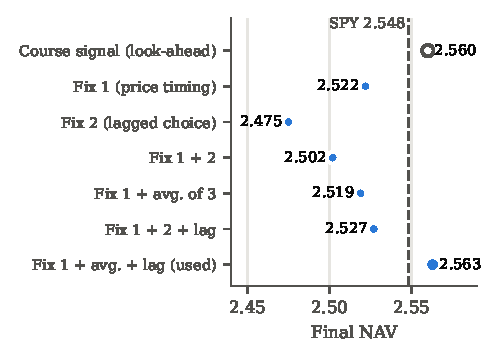
\includegraphics[width=\linewidth,height=4.8cm,keepaspectratio]{figs/fig_versions.pdf}
\end{minipage}
\caption{The same portfolio rule under each signal construction. Only one of the four leak-free
versions ends above SPY.}
\label{fig:versions}
\end{figure}

The four fully leak-free versions end between 2.50 and 2.56. The version that beats SPY was chosen
after all four were seen, so that choice was made on results, and its 0.6\% margin is far inside the
spread between them.

\subsection{Survivorship bias}
Survivorship bias means testing a strategy only on the companies that still exist today, quietly
removing every company that went bankrupt or got bought. The course's list of companies handles this
correctly: it includes Whole Foods, SVB and Activision for the years they were in the index. But the
price file only covers 501 of the 674 historical members, leaving out companies that are no longer in
the index, and the notebook gives those 173 companies a 0\% return (10.9\% of the baseline's weight on
average).

Simply skipping the stocks without prices is not a fix; it is the bias itself, and it would make the
same strategy jump from \$2.56 to \$2.86. Instead, prices for 84 of the missing companies come from
Yahoo Finance, including ones that only changed their ticker symbol. Each series is checked against
the dataset's own prices, with two special cases:
\begin{itemize}\setlength{\itemsep}{1pt}
\item Paramount's old symbol now belongs to a different security, so it is dropped.
\item SVB and First Republic are booked at a 100\% loss on the day regulators seized them.
\end{itemize}
Eighteen held names (about 5\% of the weight, mostly acquisitions such as ATVI and XLNX) still have no
price anywhere and earn 0\%. If they had earned their sectors' average return instead, the NAV would
be 2.68 rather than 2.56, so 0\% is probably conservative.

\subsection{Warm-up}
A stock only has a prediction once its company has filed a quarterly report. With the course's
original timing, only one company (Textron) had a live prediction at the first rebalance on May 1,
2020, so the ``top 25\%'' portfolio was 100\% in that one stock until more companies filed. Those first
three months returned +27.5\% against +16.0\% for the S\&P 500, so a handful of lucky stocks drove most
of the early lead. A rule was therefore added so the result does not depend on so few stocks: hold the
index until at least half of the companies in the index have a live prediction (in practice May--July
2020). With the leak-free timing, no signal is usable before July 2020; without the rule, the strategy
would sit in cash while the market rallied and end at NAV 2.20, so the rule also raises the final
result. Any threshold from 10\% to 90\% gives a NAV between 2.56 and 2.61.

\section{Stock selection}
For each sector and each rolling window, three models (Random Forest, XGBoost and LightGBM) are tuned
with grid search. In the course's original pipeline, XGBoost won 93 of the 238 sector-windows, Random
Forest won 85 and LightGBM won 60, so no single model is consistently the most accurate. The strategy
therefore averages the three instead of picking a single winner.

The course code does not save feature importances, so a proxy was trained: one pooled XGBoost model on
the periods before 2020. The importances are almost flat (inventory turnover 2.5\%, P/B 2.4\%; a
uniform split is 1.9\%), which means that no single ratio dominates the predictions.

The signal is weak: the mean quarterly rank IC between predicted and actual returns is about 0.004 for
the course's selected model and 0.020 (t = 0.62) for the three-model average used here. Neither is
statistically different from zero. The strategy keeps the notebook's top-25\% selection.

\section{Strategy and backtest}
On the first trading day of each month, at the close, the strategy ranks every live prediction across
all sectors and keeps the top 25\% of the companies, about 123 stocks.

Within that group, each stock is weighted by the rank of its prediction: the best prediction gets
about twice the median weight, and the largest position averages 1.6\%. Between rebalances, the
weights drift with prices. The strategy assumes a trading cost of 0.1\% of the amount traded; about a
third of the portfolio is traded each month, so costs add up to 2.2\% over the whole period.

The original notebook's backtest computes each stock's daily return as the closing price over the
opening price, which means buying at the open and selling at the close of the same day. In reality, a
typical portfolio holds stocks overnight and also earns the move from one day's close to the next
day's open. The notebook's SPY benchmark, on the other hand, is measured from close to close, so the
original comparison was not like for like.

How much does this matter? An equal-weight portfolio of every stock in the dataset over the same period
shows the size of the effect:
\begin{itemize}\setlength{\itemsep}{1pt}
\item Counting only open-to-close moves, \$1 grew to \$1.26.
\item Counting from close to close, it grew to \$2.78, so in this sample more than half of the return
came overnight.
\end{itemize}
The baseline therefore lost to the S\&P 500 mainly because it missed overnight returns, not because of
bad stock choices. The strategy and the benchmarks (SPY and QQQ total return, cached so the results are
reproducible) all use close-to-close returns with dividends. Rebalancing monthly instead of
re-weighting daily also roughly halves turnover (0.029 to 0.016 per day) and cuts costs from 3.9\% to
2.2\% in total.

\section{Performance}
\begin{table}[h]
\centering\small
\begin{tabular}{lrrrrrrr}
\toprule
2020-05 to 2025-09, net of 0.1\% costs & NAV & Cum.\ return & CAGR & Vol & Sharpe & Max DD & Turnover/day\\
\midrule
Baseline & 1.31 & +30.7\% & 5.1\% & 15.2\% & 0.40 & $-$19.8\% & 0.032\\
\textbf{The reported strategy} & \textbf{2.563} & \textbf{+156.3\%} & \textbf{19.0\%} & 20.7\% & 0.95 & $-$31.4\% & 0.016\\
Top 25\%, equal weight & 2.561 & +156.1\% & 19.0\% & 19.6\% & 0.99 & $-$28.4\% & 0.016\\
Sector-neutral scoring & 2.34 & +134.0\% & 17.0\% & 18.2\% & 0.96 & $-$26.5\% & 0.028\\
No-model control (all members, EW) & 2.29 & +128.9\% & 16.5\% & 16.5\% & 1.01 & $-$20.1\% & 0.006\\
\textit{Survivors only (biased)} & \textit{2.86} & \textit{+186.3\%} & \textit{21.4\%} & \textit{20.4\%} & \textit{1.06} & \textit{$-$29.5\%} & \textit{0.016}\\
SPY & 2.548 & +154.8\% & 18.9\% & 17.5\% & 1.08 & $-$24.5\% & --\\
QQQ & 2.91 & +191.5\% & 21.8\% & 23.0\% & 0.98 & $-$35.1\% & --\\
\bottomrule
\end{tabular}
\caption{Leak-free signal and warm-up rule for every row except the reproduced baseline. Sharpe uses
rf = 0.}
\label{tab:perf}
\end{table}

With all the changes in place, the final strategy buys the top 25\% of the averaged predictions each
month and gives slightly more weight to the best ones.

From May 2020 to September 2025, after trading costs, \$1 grew to \textbf{\$2.563}, while SPY grew to
\textbf{\$2.548}. The strategy beats the index by about 1.5 cents on the dollar, a negligible
advantage, and it takes more risk to get there: higher volatility, a deeper drawdown and a lower
Sharpe ratio.

After the warm-up, the strategy is ahead of SPY on 85\% of trading days; its widest deficit was 5\%, in
the April 2025 sell-off. Equal weighting does just as well with a better Sharpe, so the two rules
cannot really be told apart.

\begin{figure}[t]
\centering
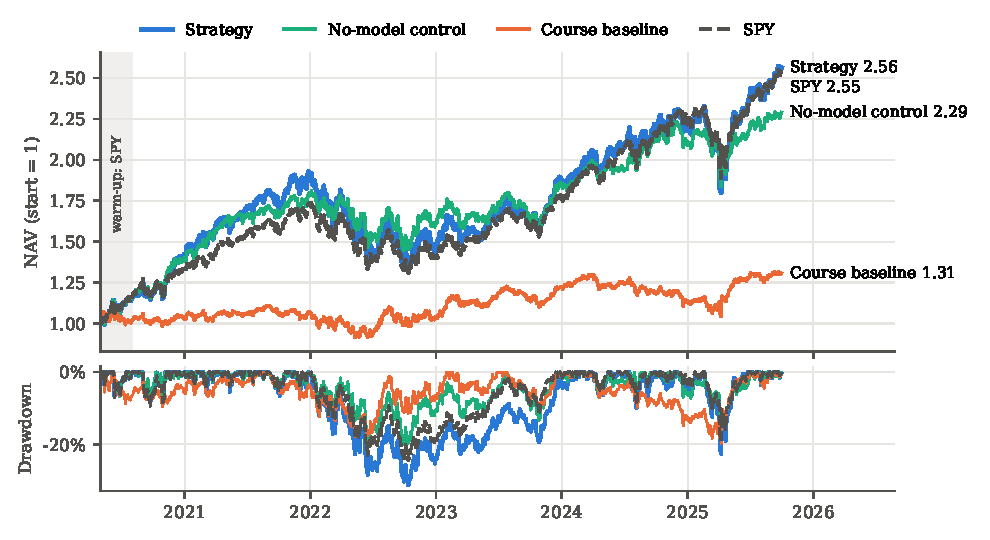
\includegraphics[width=0.78\linewidth]{figs/fig_nav.pdf}
\caption{NAV (top) and drawdown (bottom), net of costs. The shaded band is the warm-up, when every
strategy holds SPY.}
\label{fig:nav}
\end{figure}

On average, 64\% of the portfolio's money was invested in technology stocks, against 15\% when the
money is spread evenly across every stock in the index. Each sector has its own model, and the
technology model, trained on years when tech performed well, happens to predict larger returns than
the other sectors' models. Ranking all sectors' predictions on one scale therefore puts mostly tech
stocks at the top.

When each stock is ranked only against others in its own sector, the tech weight drops to 15\% and the
strategy ends at \$2.34, below the index. Most of the strategy's advantage therefore came from the
accidental bet on tech companies. Compared with the no-model control, the model adds 2.5 points of
CAGR, but only about 0.5 once scoring is sector-neutral.

\begin{figure}[ht]
\centering
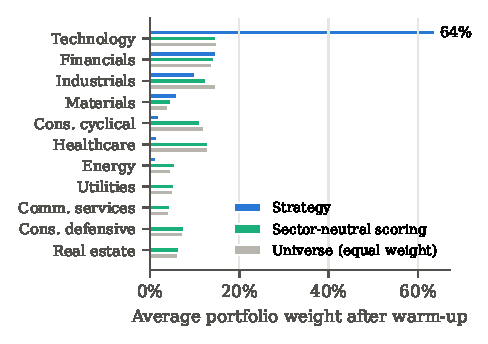
\includegraphics[width=0.42\linewidth]{figs/fig_sectors.pdf}
\caption{Average sector weights after the warm-up. Ranking predictions from 11 separately trained
sector models together produces a 64\% technology weight.}
\label{fig:sectors}
\end{figure}

\section{Robustness}
\begin{table}[htb]
\centering\footnotesize
\begin{tabular}{ll}
\toprule
Check & Result\\
\midrule
Sub-periods, CAGR (Sharpe) & 2020--22: 15.4\% (0.75) vs SPY 13.7\% (0.76); \ 2023--25: 22.7\% (1.18) vs SPY 24.2\% (1.47)\\
Excess return vs SPY & +0.7\%/yr, tracking error 7.1\%, t = 0.23 (Newey--West)\\
Market exposure & beta 1.12, alpha $-$1.5\%/yr (t = $-$0.54)\\
Multiple testing & Deflated Sharpe probability $\approx$ 3\% after $\sim$50 variants\\
Transaction costs & NAV 2.62 / 2.56 / 2.51 / 2.35 at 0 / 0.1 / 0.2 / 0.5\%; break-even $\approx$ 0.13\%\\
Validation-preferred variants & volatility weighting 2.51, retrained model 2.48, momentum blend 2.22: all below SPY\\
Literature factors & 7 anomalies, none significant; pre-2020 quality composite 2.26\\
\bottomrule
\end{tabular}
\caption{Robustness of the strategy. Validation = 2020-05 to 2022-12, test = 2023-01 to 2025-09.}
\label{tab:robust}
\end{table}

Four checks show how fragile the lead is:
\begin{itemize}\setlength{\itemsep}{1pt}
\item \textbf{Split the period} -- It won in 2020--22 (15.4\% a year vs 13.7\%) and lost in 2023--25
(22.7\% vs 24.2\%), when a few very large tech companies drove most of the index's gains.
\item \textbf{Test the significance} -- The excess return is about 0.7\% a year with a t-statistic of
0.23, suggesting the gain is not statistically significant. Beta is 1.12, so the extra return is
explained by extra market exposure.
\item \textbf{Higher risk} -- The portfolio is more volatile than the index (20.7\% vs 17.5\% a year)
and had a deeper drawdown ($-$31\% vs $-$24\%). It also earns less return per unit of risk (a Sharpe
ratio of 0.95 vs 1.08).
\item \textbf{Higher costs} -- At a 0.2\% trading cost instead of 0.1\%, the advantage is gone
(break-even is about 0.13\%).
\end{itemize}

\section{Conclusion}
The strategy meets the requirement (NAV 2.563 vs 2.548) on a sample audited for survivorship,
look-ahead and warm-up bias. However, it is not worth investing in: the margin over the index is only
about 1.5 points over the whole five-year period, and it is not statistically significant. The
strategy is also sensitive to costs and depends on an accidental tilt toward technology stocks. The
most useful outcomes of this assignment were the backtest fixes: the overnight-return fix alone
explains most of the baseline's gap to SPY, and ignoring the missing prices would have inflated the
NAV from 2.56 to 2.86.

\end{document}
